\section{Auswertung}
\label{sec:Auswertung}

\subsection{Bestimmung der Zerfallskurve und der Halbwertszeit von Indium}
Die Messdaten zur Bestimmung der Zerfallskurve und Halbwertszeit von Indium sind in Tabelle 
\ref{tab:indium} aufgetragen. 
Die Messzeit beträgt jeweils $\Delta t = \SI{240}{\second}$.
Weiterhin entspricht die Nullmessung $220$ Impulsen bei einer Messzeit von $\SI{900}{\second}$.
Damit werden immer -- durch die Übertragung auf die Messzeit $\Delta t = \SI{240}{\second}$ --
$\frac{176}{3}$ Zerfälle abgezogen.
\begin{table}
	\centering
	\caption{Messdaten der Zerfälle $N$ beim Zeitpunkt $t$ zur Bestimmung der Zerfallskurve und Halbwertszeit von Indium.}
	\label{tab:indium}
	\begin{tabular}{cc}
		\toprule
		$t$ / $\si{\second}$ & $N$ \\
		\midrule
		240 & 2576 \\
		480 & 2250 \\
		720 & 2116 \\
		960 & 1984 \\
		1200 & 1905 \\
		1440 & 1753 \\
		1680 & 1701 \\
		1920 & 1688 \\
		2160 & 1542 \\
		2400 & 1456 \\
		2640 & 1438 \\
		2880 & 1348 \\
		3120 & 1291 \\
		3360 & 1262 \\
		3600 & 1128 \\
		\bottomrule
	\end{tabular}
\end{table}
Gemäß Formel \eqref{eqn:halbwertszeit} wird die Anzahl der Zerfälle logarithmiert gegen die
Zeit aufgetragen.
Also ergibt sich der Zusammenhang
\begin{equation}
	\label{eqn:Halbwertszeit2}
	\ln N(t) = \ln N_0 - \lambda t \mathrm{.}
\end{equation}
Eine lineare Ausgleichsrechnung der Form
\begin{equation*}
	f(x) = m \cdot x + b
\end{equation*}
mit den Datentupeln $\{ t, \ln (N)\}$ aus Tabelle \ref{tab:indium} ergibt die Geradenparameter
\begin{align*}
	m &= (-\num{2,2(8)}) \cdot 10^{-4} \si{\per\second}  \, \mathrm{,} \\
	b &= \num{7,80(2)} \, \mathrm{.}
\end{align*}
Damit ist die Zerfallskonstante
\begin{equation*}
	\lambda = (\num{2,2(8)}) \cdot 10^{-4} \si{\per\second}  \, \mathrm{.} \\
\end{equation*}
Die zugehörige Ausgleichsgerade ist in Abbildung \ref{fig:indium} dargestellt.
Mit Formel \eqref{eqn:???} ergibt sich die Halbwertszeit von Indium $^{116}\mathrm{In}$
zu
\begin{equation*}
	\tau =  (\num{3.08(11)}) \cdot 10^3 \si{\second} \, \mathrm{.}
\end{equation*}
\begin{figure}
	\centering
	\includegraphics{Messdaten/indium.pdf}
	\caption{Messdaten der logarithmierten Zerfälle $N$ aufgetragen gegen die Zeit $t$ mit zugehöriger Ausgleichgerade gemäß Formel \eqref{eqn:halbwertszeit} bzw. Formel \eqref{eqn:Halbwertszeit2}.}
	\label{fig:indium}
\end{figure}






%\subsection{Untersuchung der Halbwertszeit der beiden Zerfälle bei Silber}
%Die Nullmessung bluzp
%\begin{figure}
%  \centering
%  \includegraphics{Messdaten/silber.pdf}
%  \caption{Zerfallskurve für Silber samt beider Ausgleichgraden zur Bestimmung der verschieden ablaufenden Einzelzerfälle.}
%  \label{fig:silber}
%\end{figure}
%
%\begin{figure}
%  \centering
%  \includegraphics{Messdaten/ergebnis.pdf}
%  \caption{Darstellung des mittels Ausgleichsrechnungen ermittelten summierten Zerfalls sowie der im Experiment gemessenen Werte.}
%  \label{fig:ergebnis}
%\end{figure}
%
%
%

%Bild
%\begin{figure}
%  \centering
%  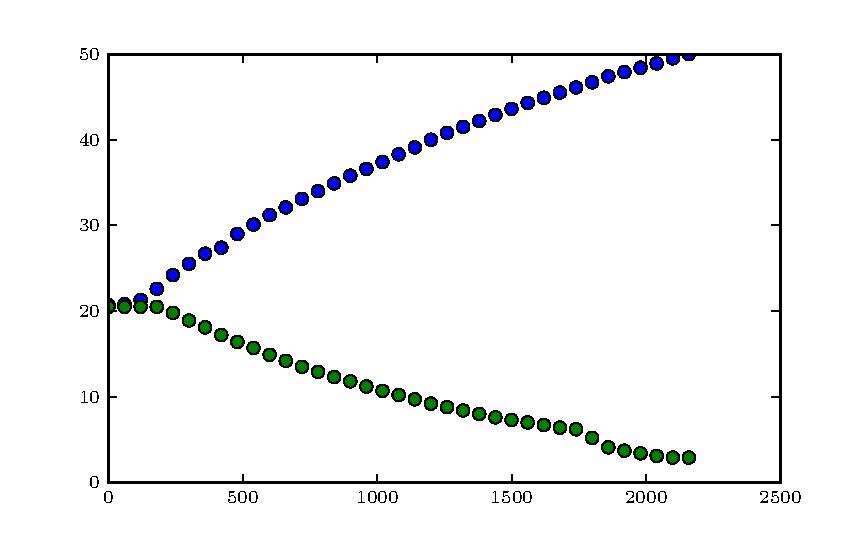
\includegraphics{plot.pdf}
%  \caption{Plot.}
%  \label{fig:plot}
%\end{figure}


%Tabelle
%\begin{table}
%	\centering
%	\caption{Table.}
%	\label{tab:table}
%	\begin{tabular}{ccc}
%		\toprule
%    column1&column2&column3\\
%		\midrule
%		220 & -391 & 659 \\
%		330 & -598 & 946 \\
%		525 & -1000 & 1660 \\
%		702 & -1337 & 2051 \\
%		930 & -1650 & 2450 \\
%		\bottomrule
%	\end{tabular}
%\end{table}
